\section{Mean-Field Background and Dropout Recursions}

\subsection{Notation Guide}
\label{app:notation}

The same few letters carry several nearby meanings, so we collect the main conventions here.
\begin{table}[h]
\caption{Notation used across the main text and appendices.}
\label{tab:notation_guide}
\centering
\small
\begin{tabular}{@{}ll@{}}
\toprule
Symbol & Meaning \\
\midrule
\(\rho_\ell\) & keep probability in layer \(\ell\) \\
\(p_{\mathrm{drop},\ell}=1-\rho_\ell\) & raw dropout probability \\
\(p_j^{(\ell)}\) & Bernoulli dropout mask variable \\
\(m=1-c^\ast\) & decorrelation order parameter at the fixed point \\
\(m_\ell=1-c_\ell\) & depth-dependent decorrelation used in relaxation laws \\
\(\chi_\perp\), \(\chi_1\) & no-dropout angular susceptibility at \(c=1\) \\
\(\chi_\rho\) & dropout-deformed angular susceptibility \(\bar F_\rho'(1)\) \\
\(\chi_M\) & response susceptibility \(\partial m/\partial h\) \\
\(\chi\), \(\chi_q\) & generic Hermite/angle susceptibility and variance-channel susceptibility \\
\(\theta_{\rm rel}\) & relaxation exponent, \(m_\ell\sim \ell^{-\theta_{\rm rel}}\) \\
\bottomrule
\end{tabular}
\end{table}
\FloatBarrier

\subsection{Mean-Field Theory Primer}
\label{app:mft_primer}

Even the Standard Model of physics, with only a few dozen empirical parameters, invites the feeling that some deeper organizing principle is yet to be found. Fermi made the same point more sharply to Dyson by quoting von Neumann: ``With four parameters I can fit an elephant, and with five I can make him wiggle his trunk'' \cite{Dyson2004Fermi}. Modern machine learning pushes this worry to an extreme: parameters are abundant, so understanding cannot mean tracking each weight individually. A pressing question in modern ML literature is what set of parameters or effective fields can give a useful description of the network's behavior, and how to derive such a description from the microscopic model.

Mean-field theory gives one such effective description: instead of tracking every neuron and every random weight, one tracks a small number of self-consistent fields. In the signal-propagation version used here, those fields are variances, covariances, and correlations. This is the deep information propagation line of mean-field theory \cite{poole2016exponentialexpressivitydeepneural,schoenholz2017deepinformationpropagation}, with broader background in statistical-mechanics treatments of deep learning \cite{Bahri2020StatMechDeepLearning,bahri2024leshoucheslecturesdeep}. The same infinite-width covariance recursion can also be read as the NNGP kernel recursion \cite{Lee2018DNNasGP}; we use the MFT language because our questions concern fixed points, susceptibilities, correlation lengths, and critical exponents rather than the induced function-space prior or training dynamics.

Section~\ref{sec:mft_background} gives the main-body version of the signal-propagation story. Here we only fix notation and record the elementary steps used later in the appendices. For a depth-$L$ MLP with activation $\phi:\mathbb R\to\mathbb R$, weights and biases are initialized as
\begin{equation}
W^{l}_{ij}\sim \mathcal{N}\left(0,\frac{\sigma_{w}^{2}}{N_{l-1}}\right), \qquad b^{l}_{i}\sim \mathcal{N}\left(0,\sigma_{b}^{2}\right),
\end{equation}
and propagated by
\begin{equation}
z^{l}_{i;a}= \sum_{j=1}^{N_{l-1}} W^{l}_{ij} y^{l-1}_{j;a}+b^{l}_{i}, \qquad y^{l}_{i;a}=\phi\left(z^{l}_{i;a}\right),
\end{equation}
where $W^l\in\mathbb R^{N_l\times N_{l-1}}$, $y^0=x$, and $a$ labels the input. We write
\begin{equation}
\int Dz (\cdots)=\frac{1}{\sqrt{2\pi}}\int_{-\infty}^{\infty}dz e^{-z^{2}/2}(\cdots),
\end{equation}
and use the same convention for multiple Gaussian variables.

The Gaussian closure comes from the fact that each preactivation is a sum of many independently initialized weighted inputs. In the infinite-width limit this central-limit effect becomes exact layer-by-layer, while finite-width corrections are organized perturbatively in the depth-to-width aspect ratio, schematically $L/N$ \cite{roberts2022principlesdeeplearningtheory}. For $l\ge2$, the single-input variance and two-input covariance recursions are the closed equations already quoted in Sec.~\ref{sec:mft_background}:
\begin{align}
q^{l}_{aa}&=\sigma_{w}^{2}\int Dz \phi^{2}\left(\sqrt{q^{l-1}_{aa}} z\right)+\sigma_{b}^{2},\nonumber\\
q^{l}_{ab}&=\sigma_{w}^{2}\int Dz_{1} Dz_{2} \phi(u_{1}) \phi(u_{2})+\sigma_{b}^{2},\nonumber\\
u_{1}&=\sqrt{q^{l-1}_{aa}} z_{1},\qquad c^{l-1}_{ab}=\frac{q^{l-1}_{ab}}{\sqrt{q^{l-1}_{aa} q^{l-1}_{bb}}},\nonumber\\
u_{2}&=\sqrt{q^{l-1}_{bb}}\left(c^{l-1}_{ab}z_{1}+\sqrt{1-\left(c^{l-1}_{ab}\right)^{2}} z_{2}\right).
\end{align}
Once the variance relaxes to $q^*$, these equations induce a one-dimensional correlation map $c^l_{ab}=F(c^{l-1}_{ab})$. Without dropout, perfect alignment is a fixed point, $F(1)=1$. Its linear stability is controlled by the angular susceptibility
\begin{equation}
\chi_{1}=\left.\frac{\partial c^{l}_{ab}}{\partial c^{l-1}_{ab}}\right|_{c_{ab}=1}=\sigma_{w}^{2}\int Dz \big[\phi'(\sqrt{q^{*}} z)\big]^{2},
\end{equation}
called $\chi_\perp$ in the main text and in \cite{roberts2022principlesdeeplearningtheory}. The ordered, chaotic, and critical regimes correspond to $\chi_1<1$, $\chi_1>1$, and $\chi_1=1$ respectively; the last case is the edge-of-chaos, where the cross-input correlation length can diverge.

The usual He initialization follows from this criterion in the special case of \relu{}. Since $\phi'(z)=\theta(z)$ almost everywhere,
\begin{equation}
\int Dz \big(\phi'(\sqrt{q^{*}}z)\big)^2=\frac12,
\qquad \chi_1=1 \Longrightarrow \sigma_w^2=2,
\end{equation}
which is the variance-$2/N$ initialization. The same example also shows why variance preservation and correlation criticality are not identical: for \relu{},
\begin{equation}
q^{l}_{aa}=\frac{\sigma_w^2}{2} q^{l-1}_{aa}+\sigma_b^2,
\end{equation}
so with nonzero bias the finite-$q^*$ condition requires $\sigma_w^2<2$, while exact angular criticality sets $\sigma_w^2=2$. In practice one either sets biases to zero or works slightly subcritical to keep the variance scale finite.

Finally, the correlation length used throughout the paper is obtained by linearizing the correlation map around its fixed point. With $r_c=F'(c^*)$ and $0<|r_c|<1$, small deviations obey
\begin{equation}
|c^*-c^l_{ab}|\propto e^{-l/\xi_c},\qquad \xi_c^{-1}=-\log|r_c|.
\end{equation}
The analogous variance length $\xi_q$ tracks relaxation of $q^l_{aa}$ to $q^*$, but the edge-of-chaos phenomenon is primarily controlled by $\xi_c$: it measures how many layers preserve distinctions between different inputs. This is the scale deformed by dropout in the main analysis.
\FloatBarrier

\subsection{Derivation of Correlation Map and Derivatives with Dropout}\label{app:price_dropout}

Fix the positive dropout-shifted variance \(\bar q^*\) from \eqref{eq:qstar-dropout}, and let \((u_1,u_2)\) be centered Gaussian with marginal variance \(\bar q^*\) and correlation \(c\). Independent inverted-dropout masks across inputs give the normalized map
\begin{equation}
\bar F_\rho(c)=\frac{\sigma_w^2\mathbb E_c[\phi(u_1)\phi(u_2)]+\sigma_b^2}{\bar q^*},
\qquad h=1-\bar F_\rho(1),
\label{eq:Frho_def_app}
\end{equation}
with \(h\) given by \eqref{eq:Delta_exact}.

Assume \(\phi\in C^2\) and \(\phi,\phi',\phi''\in L^2(\mathcal N(0,\bar q^*))\). Price's theorem \cite{Price1958GaussianInputs,Voigtlaender2021Price}, applied at fixed \(\bar q^*\), states that for \(|c|<1\),
\begin{equation}
\frac{\mathrm d^k}{\mathrm dc^k}\mathbb E_c[\phi(u_1)\phi(u_2)]
=(\bar q^*)^k\mathbb E_c[\phi^{(k)}(u_1)\phi^{(k)}(u_2)],
\qquad k=1,2.
\end{equation}
Strong continuity of Gaussian correlation operators in \(L^2\) then justifies \(c\to1^-\), giving the one-sided derivatives
\begin{align}
\bar F_\rho'(1^-)&=\sigma_w^2\int Dz\,[\phi'(\sqrt{\bar q^*}z)]^2=\chi_\rho,\\
\bar F_\rho''(1^-)&=\sigma_w^2\bar q^*\int Dz\,[\phi''(\sqrt{\bar q^*}z)]^2=g_\rho,
\end{align}
as used in Eqs.~\eqref{eq:chi_dropout}--\eqref{eq:g_dropout}. The boundary passage requires the stated Gaussian square-integrability conditions; the theorem for nondegenerate \(|c|<1\) alone does not establish finite derivatives at perfect alignment.

\FloatBarrier

\subsection{Extensions to Infinite-Channel CNNs and ResNets}
\label{app:cnn_extension}

We briefly discuss extensions to architectures not treated in the main analysis. Although our derivation is for MLPs, the universality-class mechanism is tied to the local Gaussian kernel rather than to the MLP architecture itself. Other architectures introduce additional structure that can change the exact exponents, but the qualitative smooth-versus-kinked distinction should remain when the same local channel controls the wide-limit recursion.

For example, the same local channel which appears in MLPs re-emerges in infinite-width CNNs when the number of channels is taken to infinity: preactivations at different spatial positions become jointly Gaussian across channels, and the covariance recursion composes the same bivariate Gaussian activation expectation with a linear operator that averages over convolutional filter offsets \cite{cnnslecun,xiao2018dynamicalisometrymeanfield}. In schematic form, a spatial covariance \(K^\ell_{\alpha\beta}(x,x')\) evolves as \(K^{\ell+1}=\sigma_b^2+\sigma_w^2\mathcal A[V_\phi(K^\ell)]\), where \(V_\phi\) is the scalar Gaussian channel analyzed above and \(\mathcal A\) is the convolutional averaging operator. Independent dropout shifts the single-input variance entering \(V_\phi\) as in the fully connected case, while the cross-input covariance is still controlled by the same bivariate expectation. Therefore, for an isolated leading spatial mode, convolution changes the relevant eigenvalue and mode shape but not the local smooth-versus-kinked non-analyticity: smooth activations retain the analytic Landau equation, while \relu{}-like kinks retain the \(m^{3/2}\) branch point. A complete CNN theory would promote \(m\) to a spatial covariance-mode amplitude and track boundary conditions, pooling, and degeneracies of \(\mathcal A\).

ResNets modify depth dynamics in a complementary way: skip connections can change exponential convergence to subexponential or polynomial behavior, and norms may drift rather than relax to a fixed point \cite{yang2017meanfieldresnets}. Still, the residual branch evaluates the same nonlinear Gaussian channel \(V_\phi\), so the local analytic distinction is unchanged. The tanh/\relu{} asymptotic split observed in \cite{yang2017meanfieldresnets} is consistent with our smooth/kinked classes; a dropout-deformed ResNet theory would additionally track residual-branch strength and norm drift.

\FloatBarrier

\subsection{Regularization-Reach Derivation}
\label{app:regularization_reach}

The local-stationary propagation surrogate is invariant under permutations of the depth profile \(h_\ell\), so it fixes a saturated allocation while leaving its ordering open. We propose choosing that ordering by asking how much downstream computation sees a dropout perturbation before it is absorbed, using a common background decay scale and an additive exposure model.

First apply dropout only at layer \(\ell\). Write \(\tilde y_k^{(\ell)}\) for the masked trajectory and \(y_k\) for the clean trajectory. We measure the size of the perturbation at layer \(k\) by the clean-vs.-masked angular decorrelation
\begin{equation}
\eta_k^{(\ell)}
\equiv
1-\frac{\mathbb E_p[\langle \tilde y_k^{(\ell)},y_k\rangle]}
{\sqrt{\mathbb E_p[\|\tilde y_k^{(\ell)}\|^2]\|y_k\|^2}}.
\end{equation}
Here \(\eta_k^{(\ell)}=0\) means the two trajectories are perfectly aligned at layer \(k\). Immediately after the mask,
\begin{equation}
\eta_\ell^{(\ell)}
=1-\sqrt{\rho_\ell}
=\frac{1-\rho_\ell}{2}+\mathcal O((1-\rho_\ell)^2).
\end{equation}
The dropout field used in the main text is the same small parameter up to a constant:
\begin{equation}
h_\ell=a(1-\rho_\ell)+\mathcal O((1-\rho_\ell)^2),
\qquad
a=\frac{\sigma_w^2}{q^\ast}\int Dz\,\phi^2(\sqrt{q^\ast}z),
\end{equation}
so \(\eta_\ell^{(\ell)}\propto h_\ell\) to leading order. This constant of proportionality does not affect the scheduling optimizer.

Next, we propagate this perturbation downstream. For \(k>\ell\), the clean-vs.-masked pair is governed by the same wide-limit Gaussian correlation channel as a two-input pair, up to variance-relaxation corrections. Linearizing around an ordered background fixed point gives
\begin{equation}
\eta_{\ell+r}^{(\ell)}
\simeq C h_\ell e^{-r/\xi_c},
\end{equation}
where \(r\) is the number of downstream layers and \(C\) is independent of \(h_\ell\) to leading order. Here $\xi_c$ is the background correlation length, held fixed across mask locations. At an exactly critical clean channel the linear multiplier is one, and higher-order terms produce algebraic relaxation. If we only looked at the final readout, we would get \(C h_\ell e^{-(L-\ell)/\xi_c}\). This is larger for later dropout, because late perturbations have fewer layers over which to decay. That is why readout variance is not the object that explains front-loading.

For scheduling, we use the amount of downstream computation exposed to the mask as a proxy for regularization. We assume that a later layer's exposure is proportional to the remaining mask-induced decorrelation and add these exposures across layers. This assumption does not establish a corresponding improvement in generalization, and interactions between several masks or changes during training may alter it. We denote this cumulative exposure by \(\mathcal D_\ell\). It is not additional dropout strength; it is the downstream sum of the remaining perturbations, proportional to \(\sum_{r=1}^{L-\ell}\eta_{\ell+r}^{(\ell)}\).

Substituting the exponential decay into this exposure sum gives
\begin{equation}
\mathcal D_\ell
\;\propto\;
h_\ell\sum_{r=1}^{L-\ell}e^{-r/\xi_c}
\;\approx\;
h_\ell\int_0^{L-\ell}e^{-s/\xi_c}\,ds
\;=\;
h_\ell\xi_c\left(1-e^{-(L-\ell)/\xi_c}\right)
\;\equiv\;
h_\ell w_\ell.
\end{equation}
The approximation replaces the discrete sum by its continuum integral; using the exact geometric sum changes only constants and leaves the same monotone ordering. The weight \(w_\ell=\xi_c(1-e^{-(L-\ell)/\xi_c})\) decreases with \(\ell\): earlier masks are visible to more downstream layers before they are absorbed (Fig.~\ref{fig:regularization_reach}).

 Within the propagation surrogate, every permutation of the same saturated dropout set pays the same cost. We choose the permutation that gives the largest downstream exposure under the preceding assumptions:
\begin{equation}
\max_{\{h_\ell\}}\sum_{\ell=1}^L h_\ell w_\ell
\qquad
\text{s.t.}
\qquad
\sum_{\ell=1}^L h_\ell=L\bar h,
\qquad
0\le h_\ell\le h_{\max}.
\end{equation}
This is a linear program. Since \(w_1>w_2>\cdots>w_L\), it is solved by filling the largest weights first:
\begin{equation}
h_\ell^\star=
\begin{cases}
h_{\max}, & 1\le \ell\le k,\\
r, & \ell=k+1\le L,\\
0, & \ell>k+1,
\end{cases}
\qquad
k=\left\lfloor\frac{L\bar h}{h_{\max}}\right\rfloor,
\quad r=L\bar h-kh_{\max}.
\end{equation}
The residual $r$ enforces the budget when $L\bar h/h_{\max}$ is not an integer. This exposure model selects a front-loaded step. It predicts that sliding a fixed saturated block $B$ toward later layers reduces $\sum_{\ell\in B}w_\ell$; whether performance follows that ordering is an empirical test of the heuristic.

\begin{figure}[t]
\centering
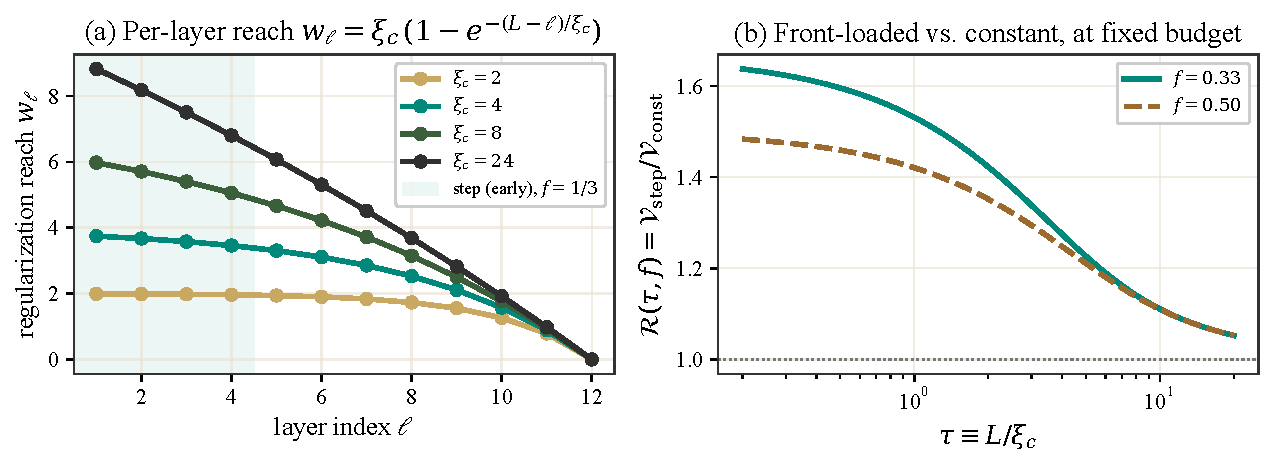
\includegraphics[width=\linewidth]{figures/theory/regularization_reach.pdf}
\caption{Regularization-reach weights at fixed network depth \(L=12\). (a)~Per-layer weight \(w_\ell=\xi_c(1-e^{-(L-\ell)/\xi_c})\) is monotone decreasing in \(\ell\) for any \(\xi_c\); the linear program over the dropout budget therefore fills the smallest-\(\ell\) layers first (shaded: step-early with \(f=1/3\)). For \(L\ll\xi_c\) the reach is essentially linear in \(L-\ell\); for \(L\gg\xi_c\) it saturates at \(\xi_c\). (b)~Ratio \(\mathcal R(\tau,f)=\mathcal V_{\rm step}/\mathcal V_{\rm const}\) of front-loaded to constant schedules at fixed budget, with \(\tau\equiv L/\xi_c\). Here $\mathcal V$ denotes summed exposure at a common background $\xi_c$. In this continuum comparison the ratio approaches $2-f$ as $\tau\to0$ and one as $\tau\to\infty$.}
\label{fig:regularization_reach}
\end{figure}

\FloatBarrier
